\chapter{Resultate} \label{resultate}
	Eine Reihe an Versuchen sollte die Möglichkeiten und Grenzen von SfM und MvS Verfahren, insbesondere von \dronarch\ aufzeigen. Sämtliche hier präsentierte Resultate wurden mit \dronarch\ gemacht und PhotoScan\autorefu{app:photoscan} wurde zur Kontrolle der Ergebnisse verwendet, vor allem wenn eine Rekonstruktion misslang.
	
	\section{Fallstudien}\label{res:fall}
		Der Versuche sollte möglichst nahe am archäologischen Anwendungsgebiet liegen, weshalb der Versuchsorte, der im folgenden Abschnitt diskutiert wird, ausgewählt wurde.

		\subsection{Gallorömisches Theater Bern Engehalbinsel}
			Durch seine klare und gut sichtbare oberirdische Struktur eignet sich das gallorämische Theater des Vicus Brenodurum auf der Engehalbinsel bei Bern gut für einen 3D Rekonstruktion mittels SfM.
			
			Aufgrund von Terra-Sigilata und Münzen, die während einer Grabung im Jahre 1956 gefunden wurden, geht man davon aus, dass die Erbauung des Theaters in die zweite Hälfte des 2.Jh. n.Chr. datiert. Die heute sichtbaren Mauern umfassen eine Fläche von etwa 35 auf 25 Meter und weist eine Höhe bis zu 1.5 Meter auf\citeu{engehalb}.	
							
			\subsubsection{3D Modell}
				Die Fotos wurden mit einer Kompaktkamera und einer Auflösung von ca. 3000px auf 2000px von Hand und mit automatischer Einstellung in weniger als 10 Minuten Arbeit erfasst.
				\dronarch\ benötigte knapp 10h für den SfM Schritt, mit dem eine Sparse Point Cloud erstellt wurde\autorefu{amphi_sparse}.
				In weiteren 7h Rechenzeit wurde mittels MvS eine Point Cloud von 7 mio Punkten erstellt, die nach grober Bearbeitung auf 4 mio Punkte reduziert wurde\autorefu{amphi_dense}.

			\subsubsection{Beobachtungen}
				\begin{figure}
					\vspace*{-4cm}
					\begin{subfigure}{\textwidth}
						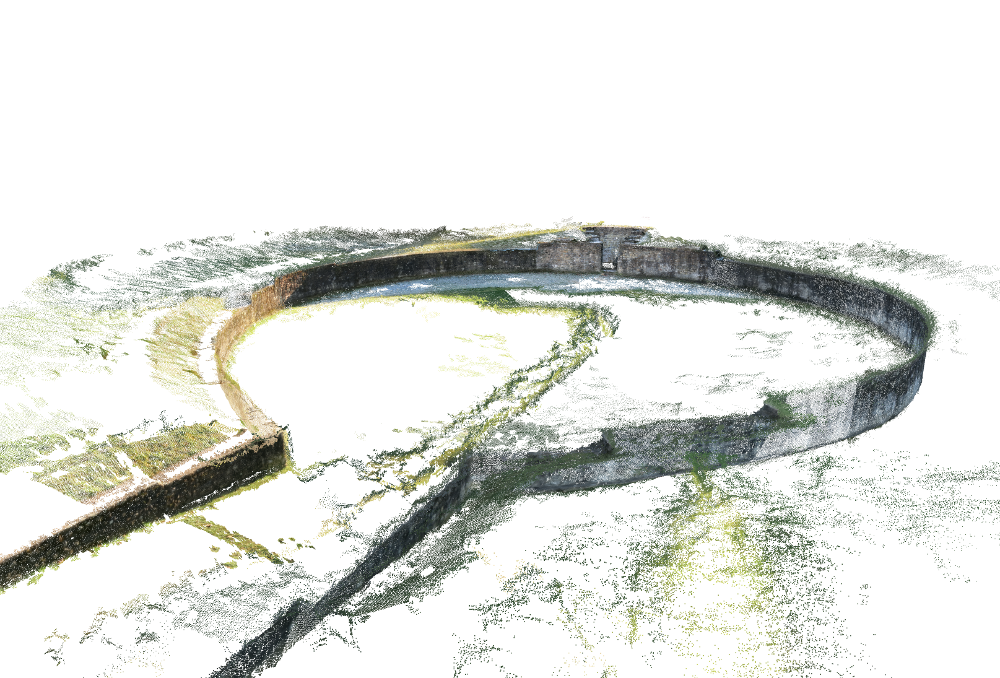
\includegraphics[width=\textwidth]{amphi_meshlab_01_sm}
						\caption{Die Mauern weisen viele Punkte auf, die Fläche in der Mitte bleibt leer.}
						\label{amphi_res_1}
					\end{subfigure}
					\begin{subfigure}{\textwidth}
						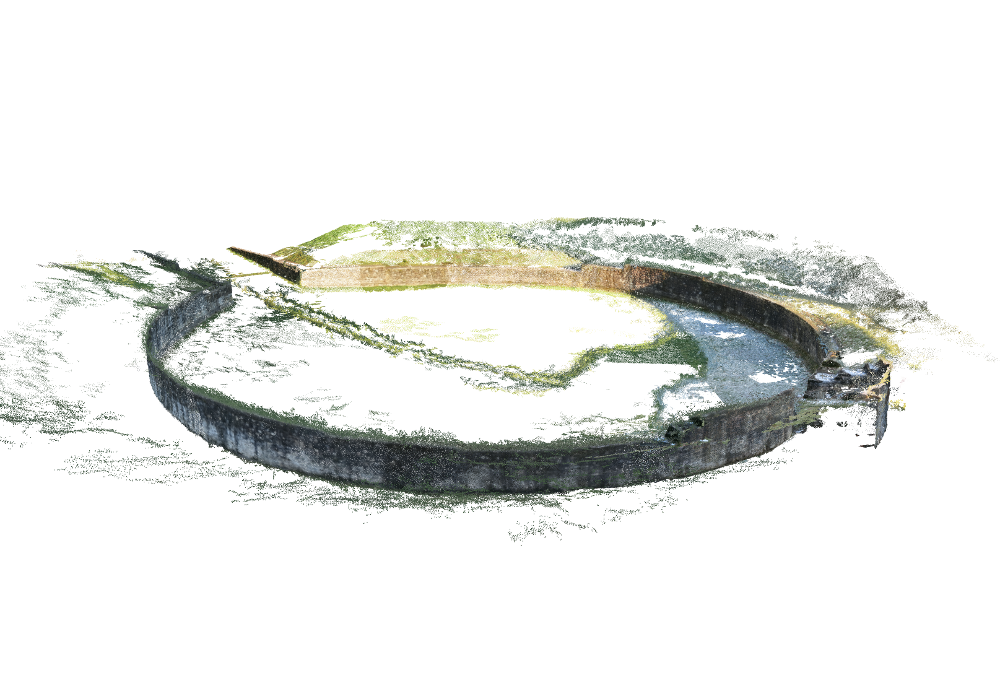
\includegraphics[width=\textwidth]{amphi_meshlab_02_sm}
						\caption{}
						\label{amphi_res_2}
					\end{subfigure}
					\begin{subfigure}{\textwidth}
						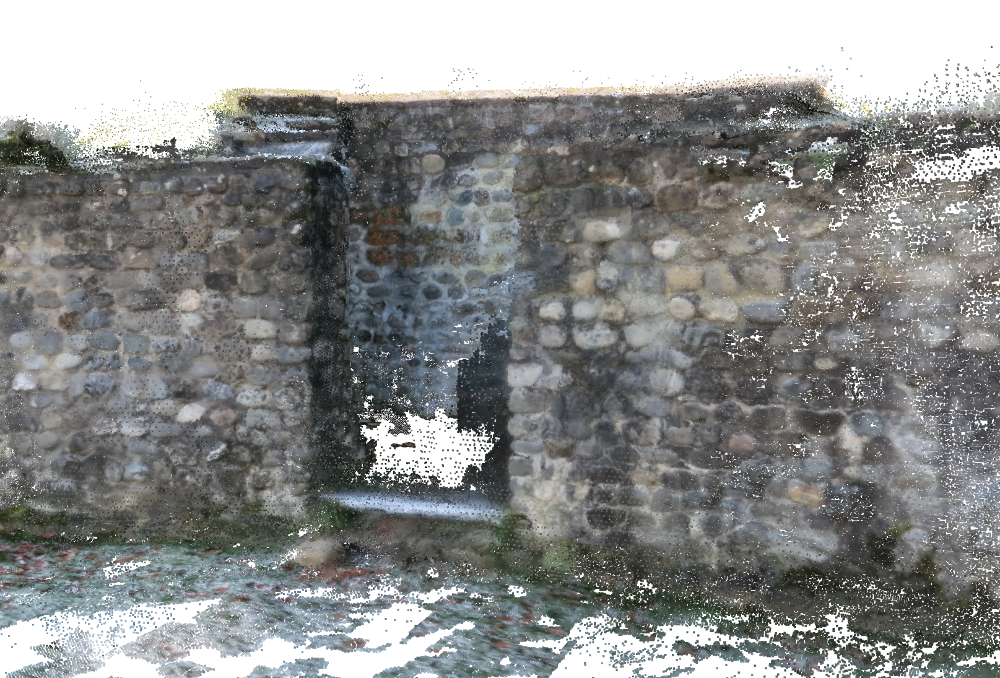
\includegraphics[width=\textwidth]{amphi_meshlab_03_sm}
						\caption{Detailansicht. Eine Ecke war auf keinem Foto sichtbar, es fehlen deshalb Punkte.}
						\label{amphi_res_3}
					\end{subfigure}
					\caption{Dense Point Clouds des gallorämischen Theaters Engehalbinsel}
					\label{amphi_res}
				\end{figure}
				Die Point Cloud ist an Stellen mit optisch auffälliger Struktur, etwa die Mauer selbst, sehr detailreich und exakt\autorefu{amphi_res_1}. In uniformen Gegenden, wie dem Rasen in der Mitte, sind fast keine Punkte vorhanden\autorefu{amphi_res_2}, was das erstellen eines Meshs enorm erschwert.
								
				Bei den Mauern ist zu beobachten, dass der Detailgrad nicht gleichmässig ist. Stellen, die auf den Fotos mehr Details aufweisen, sind auch in der Rekonstruktion deutlich besser\autorefu{amphi_res_3}.
				Einige Stellen sind auf keinem Foto sichtbar, die Rekonstruktion schlägt dort komplett fehl.
				
				\autoref{ortho_amphi_meshlab} zeigt einen Vergleich einer orthogonale Projektion des Modells mit einem Plan des Theaters. Er zeigt nur kleine Abweichungen auf, die eher auf die manuelle Orientierung und Positionierung der Bilder zurückzuführen ist als auf einen Fehler im Modell.
				\begin{figure}
					\begin{subfigure}{0.4\textwidth}
						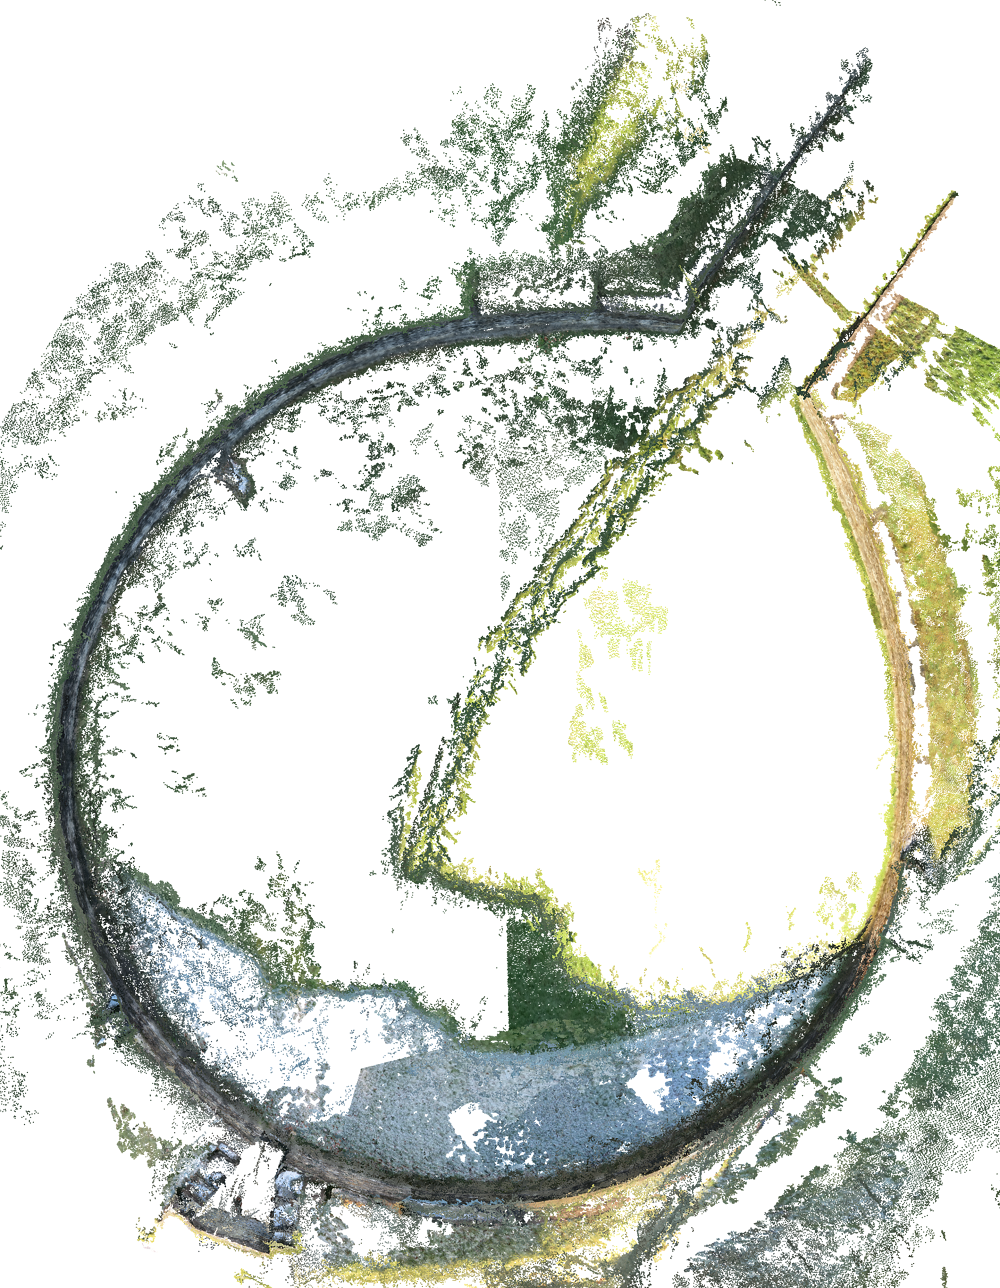
\includegraphics[width=\textwidth]{amphi_ortho_meshl_sm}
						\caption{Orthofoto der Point Cloud}
					\end{subfigure}	
					\begin{subfigure}{0.4\textwidth}
						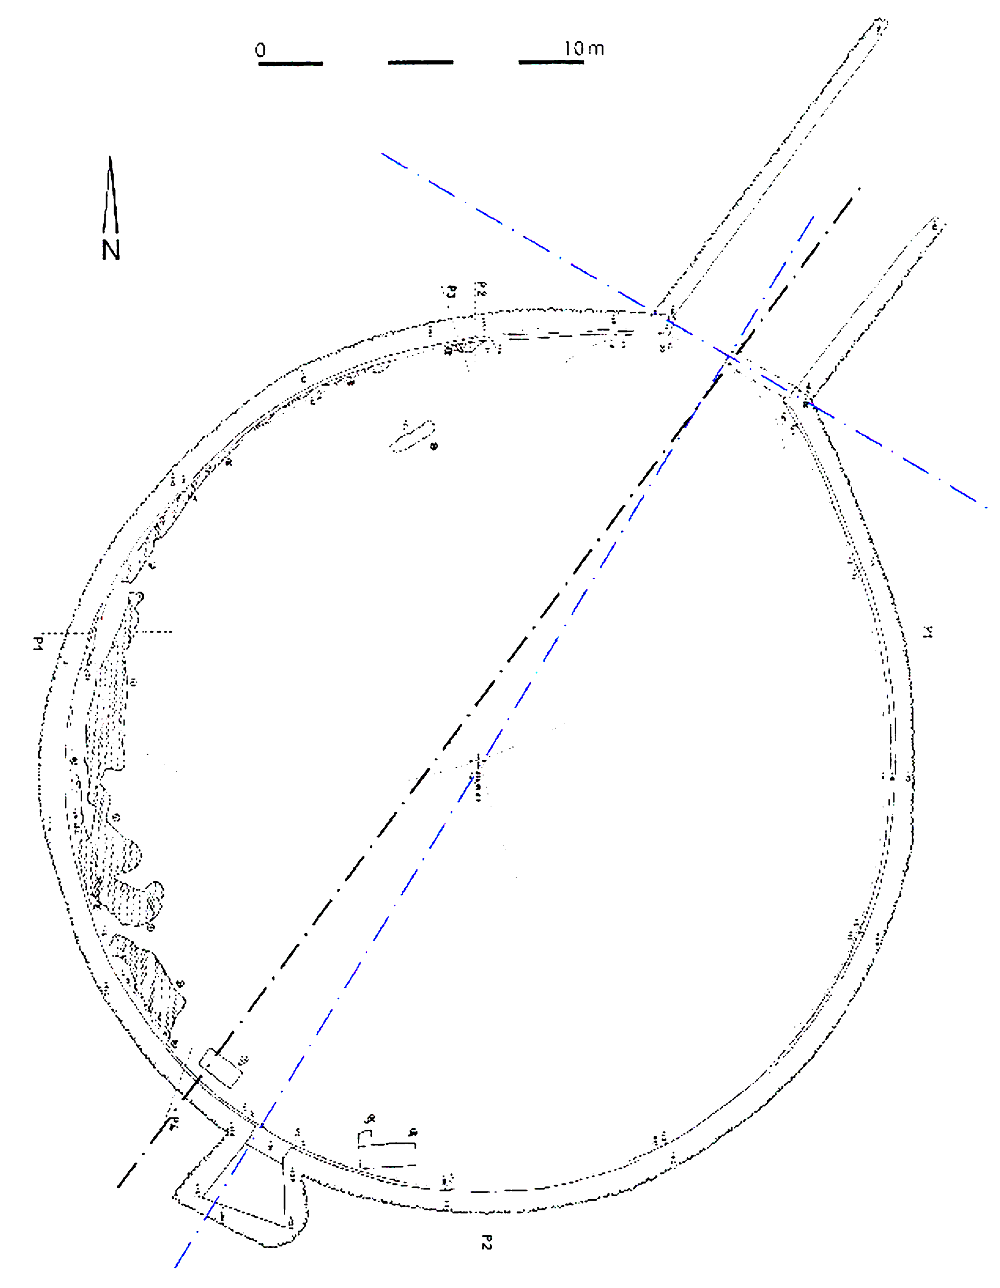
\includegraphics[width=\textwidth]{amphi_ortho_plan_edit_sm}
						\caption{Plan des Theaters}
					\end{subfigure}
					\begin{subfigure}{\textwidth}
						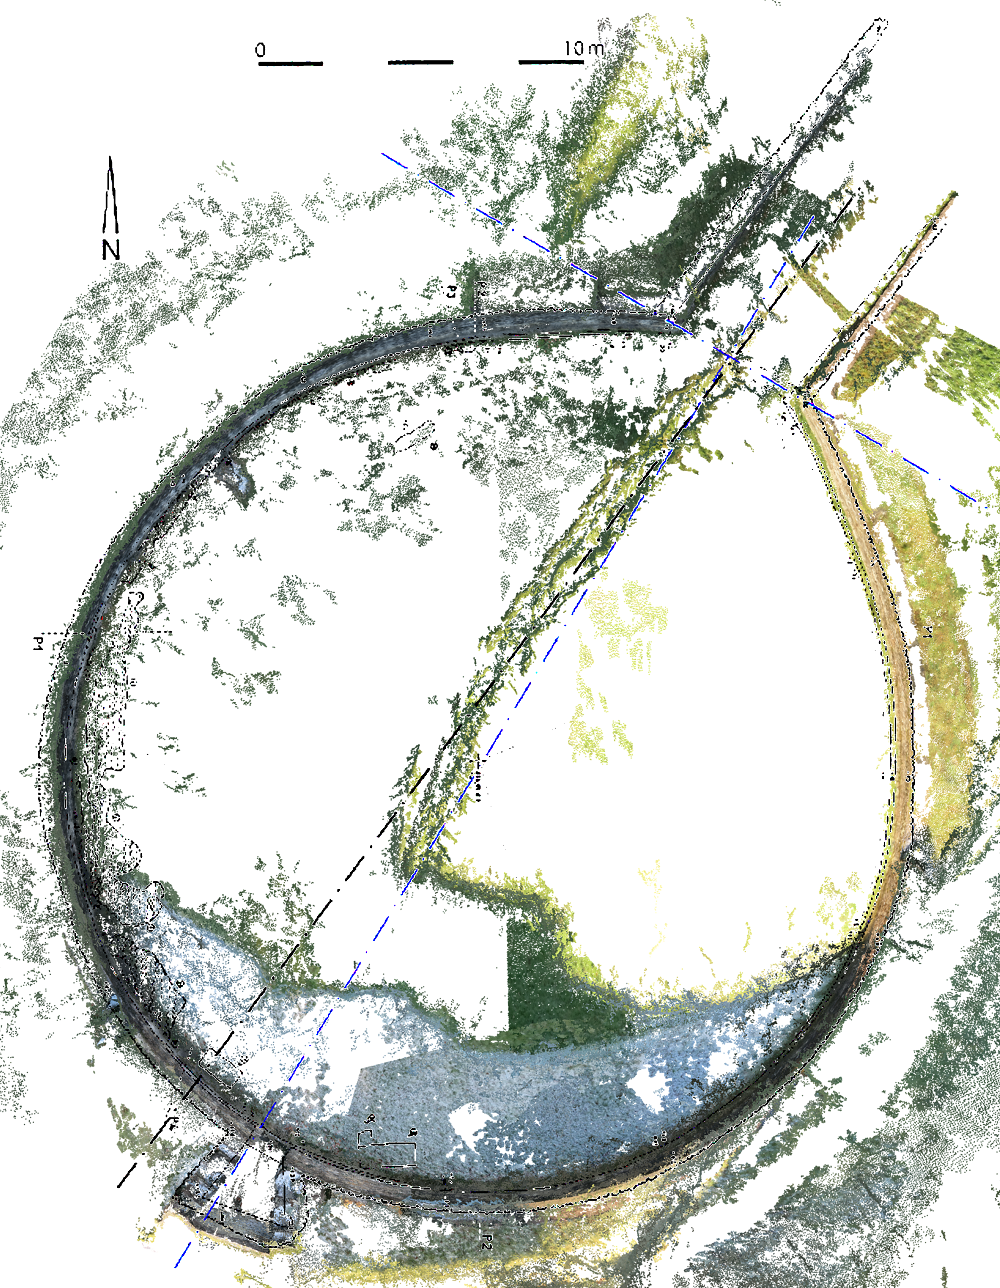
\includegraphics[width=\textwidth]{amphi_ortho_mesh_sm}
					\end{subfigure}
					\caption[Überlagerung von Plan und Orthofoto. Plan aus \cite{engehalb}]{Überlagerung von Plan und Orthofoto. Die Abweichung ist unten links ersichtlich.}
					\label{ortho_amphi_meshlab}
				\end{figure}
				
%		\subsection{Test mit vorhandenen Bildern} \label{res:test_vorhandene_bilder}
%			TODO: Welche Bilder?
			
	\section{Scans kleiner Objekte}
		SfM erscheint auch attraktiv um einzelne kleine Objekte, wie Knochen oder Keramikfragmente, 3D zu erfassen und dokumentieren. In sieben Versuchen mit verschiedenen Objekten ist es allerdings weder mit \dronarch\ noch mit PhotoScan\autorefu{app:photoscan} gelungen eine vollständige Rekonstruktion zu machen. Deshalb kann das Verfahren auf kleine Objekte angewendet so nicht als brauchbare Alternative zu Laserscannern betrachtet werden
		